\chapter{अपचयोपचय साम्य और नेर्न्स्ट समीकरण}\label{ch:b1:nernst}

ज़िंक सल्फ़ेट के विलयन में ज़िंक की एक पट्टी रखिए, कॉपर(II) सल्फ़ेट के विलयन में
कॉपर की पट्टी, दोनों विलयनों को लवण-विलयन की एक नली से जोड़िए और दोनों धातुओं को
एक प्रकाश-उत्सर्जक डायोड से होकर जाने वाले तार से: डायोड जल उठता है। ज़िंक और कॉपर
आयनों की अभिक्रिया, जो एक ही बीकर में केवल विलयन को गर्म करती है, अब इलेक्ट्रॉनों को
तार से होकर धकेलती है। बैटरी यही व्यवस्था है, पैक की हुई; pH मीटर और क्लोराइड
इलेक्ट्रोड इसके मापने वाले भाई-बंधु हैं। यह अध्याय इलेक्ट्रॉन
विनिमय को मात्रात्मक बनाता है: इलेक्ट्रॉन गिनने के लिए \omterm{def:b1:nernst:oxidation-number}{ऑक्सीकरण संख्याएँ},
युग्मों को क्रम देने के लिए \omterm{def:b1:nernst:electrode-potential}{इलेक्ट्रोड विभव}, और सांद्रता के साथ उनका अनुसरण करने के लिए
\omterm{thm:b1:nernst:nernst}{नेर्न्स्ट समीकरण}।

\begin{recall}
विद्यालय के खंड (कक्षा 11 और 12) ने \omterm{def:b1:nernst:couple}{ऑक्सीकारकों} और \omterm{def:b1:nernst:couple}{अपचायकों} को परिभाषित किया था,
\omterm{def:b1:nernst:couple}{अर्ध-समीकरण} लिखे थे, दो धातुओं और दो विलयनों से सेल बनाए थे और
ज़िंक--कॉपर सेल को बैटरी के रूप में पढ़ा था। \omterm{def:b1:extent-q-and-k:quotient}{अभिक्रिया भागफल} और
साम्य स्थिरांक \cref{ch:b1:extent-q-and-k} वाले ही हैं; \omterm{def:b1:extent-q-and-k:activity}{सक्रियताएँ}
विलेयों के लिए $c/c^\circ$ और गैसों के लिए $p/p^\circ$ हैं, शुद्ध ठोसों
और द्रवों के लिए 1।
\end{recall}

\section{ऑक्सीकरण संख्याएँ और युग्म}

\begin{definition}[ऑक्सीकारक, अपचायक, अपचयोपचय युग्म, अर्ध-समीकरण]\label{def:b1:nernst:couple}
\emph{ऑक्सीकारक}\index{ऑक्सीकारक} वह स्पीशीज़ है जो इलेक्ट्रॉन ग्रहण कर सकती है,
\emph{अपचायक}\index{अपचायक} वह जो उन्हें दे सकती है। कोई ऑक्सीकारक
Ox और वह अपचायक Red जो यह बनता है, एक \emph{अपचयोपचय
युग्म}\index{अपचयोपचय युग्म} Ox/Red बनाते हैं, जिसका वर्णन उसके
\emph{अर्ध-समीकरण}\index{अर्ध-समीकरण}
$\alpha\,\mathrm{Ox} + n\,\mathrm{e^-} \rightleftharpoons
\beta\,\mathrm{Red}$ से होता है, जो आवश्यकता होने पर \ce{H2O} और \ce{H+} से परमाणुओं में
और इलेक्ट्रॉनों से आवेश में संतुलित किया जाता है।
\end{definition}

अपचयोपचय अभिक्रिया दो युग्मों के बीच इलेक्ट्रॉनों का विनिमय है: एक का
\omterm{def:b1:nernst:couple}{ऑक्सीकारक} अपचित होता है जबकि दूसरे का \omterm{def:b1:nernst:couple}{अपचायक} ऑक्सीकृत होता है,
और इलेक्ट्रॉन कट जाते हैं। किसी जटिल स्पीशीज़ में उन्हें गिनने के लिए हर
परमाणु को एक \omterm{def:b1:nernst:oxidation-number}{ऑक्सीकरण संख्या} दी जाती है।

\begin{definition}[ऑक्सीकरण संख्या]\label{def:b1:nernst:oxidation-number}
किसी स्पीशीज़ में किसी परमाणु की \emph{ऑक्सीकरण संख्या}\index{ऑक्सीकरण संख्या}
वह आवेश है जो उस पर होता यदि हर आबंध इस तरह तोड़ा जाए कि
दोनों आबंधी इलेक्ट्रॉन अधिक विद्युत-ऋणात्मक परमाणु को मिलें (दो सर्वसम
परमाणुओं के बीच बराबर बँटें)। इसे रोमन अंकों में लिखा जाता है: आयरन(III),
परमैंगनेट आयन में \ce{Mn^{+VII}}।
\end{definition}

\begin{proposition}[ऑक्सीकरण संख्याओं के नियम]\label{prop:b1:nernst:on-rules}
\begin{enumerate}
  \item तत्व में किसी परमाणु की \omterm{def:b1:nernst:oxidation-number}{ऑक्सीकरण संख्या} 0 होती है; एकपरमाणुक आयन की
        उसका आवेश।
  \item किसी स्पीशीज़ के परमाणुओं की \omterm{def:b1:nernst:oxidation-number}{ऑक्सीकरण संख्याओं} का योग उसके
        आवेश के बराबर होता है।
  \item हाइड्रोजन $+$I होता है (धातु हाइड्राइडों को छोड़कर, जहाँ $-$I); ऑक्सीजन
        $-$II (परॉक्साइडों को छोड़कर, जहाँ $-$I, और फ़्लुओरीन से बँधे होने पर); फ़्लुओरीन
        $-$I।
  \item \omterm{def:b1:nernst:couple}{अर्ध-समीकरण} में इलेक्ट्रॉनों की संख्या बदलने वाले तत्व की \omterm{def:b1:nernst:oxidation-number}{ऑक्सीकरण संख्या} के
        परिवर्तन और उसके परमाणुओं की संख्या के
        गुणनफल के बराबर होती है।
\end{enumerate}
\end{proposition}

\begin{proof}
1 और 2: सभी आबंध तोड़ने से आवेश संरक्षित रहता है, और सर्वसम परमाणुओं के बीच
कुछ स्थानांतरित नहीं होता। 3: हाइड्रोजन उन सभी अधातुओं से कम विद्युत-ऋणात्मक है
जिनसे वह आबंधित होता है (\cref{ch:b1:periodicity}) और क्षार
धातुओं से अधिक; ऑक्सीजन फ़्लुओरीन को छोड़कर हर तत्व से अधिक विद्युत-ऋणात्मक है,
और \ce{O-O} में साझा युग्म बँट जाता है। 4: H और O अपनी संख्याएँ बनाए रखते हैं,
इसलिए केवल संबंधित तत्व के परमाणुओं का काल्पनिक आवेश बदलता है,
और इलेक्ट्रॉन \omterm{def:b1:nernst:couple}{अर्ध-समीकरण} में ठीक उतने आते हैं जितने आवेश के उस परिवर्तन को
संतुलित करने के लिए चाहिए।
\end{proof}

\begin{method}[किसी स्पीशीज़ की ऑक्सीकरण संख्याएँ]\label{met:b1:nernst:oxidation-numbers}
H, O, F और आयनों को उनकी सामान्य संख्याएँ दीजिए; बचे हुए
परमाणु की संख्या नियम 2 से निकलती है। \ce{MnO4-} में: $x + 4(-2) = -1$, $x = +7$।
\ce{Cr2O7^2-} में: $2x - 14 = -2$, $x = +6$। \ce{S4O6^2-} में औसत
$+2.5$ है; \omterm{def:b1:lewis-resonance-vsepr:lewis}{लुइस संरचना} दो प्रकार के सल्फ़र दिखाती है।
\end{method}

\begin{method}[अर्ध-समीकरण संतुलित करना]\label{met:b1:nernst:balance-by-on}
\begin{enumerate}
  \item \omterm{def:b1:nernst:oxidation-number}{ऑक्सीकरण संख्या} बदलने वाले तत्व को संतुलित कीजिए।
  \item इलेक्ट्रॉन जोड़िए: \omterm{def:b1:nernst:oxidation-number}{ऑक्सीकरण संख्या} का परिवर्तन गुणा
        परमाणुओं की संख्या।
  \item आवेश को \ce{H+} (अम्लीय विलयन) या \ce{OH-}
        (क्षारकीय विलयन) से संतुलित कीजिए।
  \item हाइड्रोजन और ऑक्सीजन को \ce{H2O} से संतुलित कीजिए; ऑक्सीजन की जाँच अंत में कीजिए।
\end{enumerate}
अम्ल में परमैंगनेट आयन के लिए: Mn $+$VII से $+$II पर जाता है, इसलिए 5
इलेक्ट्रॉन; बाईं ओर आवेश $-1 - 5 = -6$ है और दाईं ओर $+2$,
इसलिए $8\,\ce{H+}$; फिर $4\,\ce{H2O}$:
\ce{MnO4- + 8H+ + 5e- -> Mn^2+ + 4H2O}।
\end{method}

\section{विद्युत-रासायनिक सेल}

\begin{definition}[विद्युत-रासायनिक सेल]\label{def:b1:nernst:cell}
\emph{विद्युत-रासायनिक सेल}\index{विद्युत-रासायनिक सेल} दो
\emph{अर्ध-सेल}\index{अर्ध-सेल} हैं, हर एक एक युग्म और एक
इलेक्ट्रॉनिक चालक, यानी इलेक्ट्रोड, से बना, जो एक आयनिक चालक से जुड़े हों, प्रायः
\emph{लवण सेतु}\index{लवण सेतु} से (पोटैशियम नाइट्रेट जैसे किसी अक्रिय लवण के
सांद्र विलयन का जेल या नली)। जिस इलेक्ट्रोड पर ऑक्सीकरण
होता है वह \emph{ऐनोड}\index{ऐनोड} है, जिस पर अपचयन
होता है वह \emph{कैथोड}\index{कैथोड}। \emph{सेल
वोल्टता}\index{सेल वोल्टता} दोनों इलेक्ट्रोडों के बीच विद्युत विभव का
अंतर है, धन ध्रुव ऋण ध्रुव, जो
धारा न बहते समय मापा जाता है।
\end{definition}

\begin{omfigure}
\begin{tikzpicture}[font=\small, >={Stealth}]
  \pic at (0,0) {beaker={0.7}{omDef!14}};
  \pic at (3.6,0) {beaker={0.7}{omDef!32}};
  \pic at (-0.3,0.25) {electrode={black!35}};
  \pic at (3.9,0.25) {electrode={orange!70!brown}};
  \pic at (0.35,0.55) {saltbridge={2.9}};
  \pic (m) at (1.8,4.3) {meter={V}};
  \draw[thick] (-0.15,2.65) |- (m-a);
  \draw[thick] (4.05,2.65) |- (m-b);
  \node[anchor=east] at (-0.95,1.0) {\ce{Zn}};
  \node[anchor=west] at (4.45,1.0) {\ce{Cu}};
  \node at (0.25,-0.35) {\ce{Zn^2+}, \ce{SO4^2-}};
  \node at (3.6,-0.35) {\ce{Cu^2+}, \ce{SO4^2-}};
  \draw[->, omProp, thick] (-0.15,3.35) -- (0.8,3.35) node[above, midway] {$\mathrm{e^-}$};
  \draw[->, omProp, thick] (2.8,3.35) -- (3.75,3.35) node[above, midway] {$\mathrm{e^-}$};
  \node[anchor=east] at (-0.9,2.3) {$-$ ऐनोड};
  \node[anchor=west] at (4.6,2.3) {कैथोड $+$};
  \node[font=\scriptsize, align=center] at (1.8,2.75) {लवण सेतु\\ \ce{K+} $\rightarrow$ \quad $\leftarrow$ \ce{NO3-}};
  \node[font=\scriptsize] at (-0.1,-0.8) {\ce{Zn -> Zn^2+ + 2e-}};
  \node[font=\scriptsize] at (3.7,-0.8) {\ce{Cu^2+ + 2e- -> Cu}};
\end{tikzpicture}

{\small ज़िंक--कॉपर (डेनियल) सेल। ज़िंक \omterm{def:b1:nernst:cell}{ऐनोड} पर ऑक्सीकृत होता है,
जो ऋण ध्रुव है; कॉपर आयन \omterm{def:b1:nernst:cell}{कैथोड} पर अपचित होते हैं, जो धन
ध्रुव है। इलेक्ट्रॉन बाहरी परिपथ से ज़िंक से कॉपर की ओर बहते हैं;
\omterm{def:b1:nernst:cell}{लवण सेतु} में धनायन \omterm{def:b1:nernst:cell}{कैथोड} की ओर और ऋणायन
\omterm{def:b1:nernst:cell}{ऐनोड} की ओर चलते हैं, जिससे हर विलयन उदासीन बना रहता है।}
\end{omfigure}

सेल को एक पंक्ति के रूप में लिखा जाता है, \omterm{def:b1:nernst:cell}{ऐनोड} बाईं ओर: \ce{Zn} $|$ \ce{Zn^2+}
$\|$ \ce{Cu^2+} $|$ \ce{Cu}, अंतरापृष्ठों के लिए एकल रेखाएँ, \omterm{def:b1:nernst:cell}{लवण सेतु} के लिए
दोहरी रेखा। सभी सांद्रताएँ \qty{1}{mol/L} पर हों तो इसकी
वोल्टता \qty{1.10}{V} होती है। जब सेल धारा देता है तब चलने वाली अभिक्रिया,
\ce{Zn + Cu^2+ -> Zn^2+ + Cu}, वही है जो एक ही बीकर में होती;
\omterm{def:b1:nernst:cell}{अर्ध-सेलों} को अलग करना इलेक्ट्रॉनों को तार से होकर जाने के लिए विवश करता है,
जहाँ वे कार्य कर सकते हैं।

\section{इलेक्ट्रोड विभव}

वोल्टता एक अंतर है: केवल दो \omterm{def:b1:nernst:cell}{अर्ध-सेलों} के बीच के अंतर ही मापे जा
सकते हैं। इसलिए एक संदर्भ \omterm{def:b1:nernst:cell}{अर्ध-सेल} सदा के लिए चुन लिया जाता है।

\begin{definition}[इलेक्ट्रोड विभव, मानक विभव]\label{def:b1:nernst:electrode-potential}
\emph{मानक हाइड्रोजन इलेक्ट्रोड}\index{मानक हाइड्रोजन इलेक्ट्रोड}
एक प्लैटिनम इलेक्ट्रोड है जो \qty{1}{bar} पर हाइड्रोजन गैस और
\omterm{def:b1:extent-q-and-k:activity}{सक्रियता} 1 वाले \ce{H+} के आदर्श विलयन के संपर्क में है। किसी \omterm{def:b1:nernst:cell}{अर्ध-सेल} का \emph{इलेक्ट्रोड
विभव}\index{इलेक्ट्रोड विभव} $E$ उस सेल की वोल्टता है
जो बाईं ओर मानक हाइड्रोजन इलेक्ट्रोड के साथ बनता है:
$E = V_{\text{अर्ध-सेल}} - V_{\text{SHE}}$। जब युग्म की हर स्पीशीज़ की
\omterm{def:b1:extent-q-and-k:activity}{सक्रियता} 1 हो, तो यह युग्म का \emph{मानक विभव}\index{मानक विभव}
$E^\circ$ है, जो किसी दिए गए ताप पर एक स्थिरांक है।
\end{definition}

\begin{omfigure}
\begin{tikzpicture}[font=\small, >={Stealth}]
  \pic at (0,0) {beaker={0.72}{omDef!14}};
  % glass jacket, open at the bottom, with the gas inlet on the right
  \draw[om glass] (-0.32,0.35) -- (-0.32,3.0) -- (0.32,3.0) -- (0.32,2.55)
    -- (0.95,2.55) (0.32,2.35) -- (0.95,2.35) (0.32,2.35) -- (0.32,0.35);
  \draw[thick] (0,0.9) -- (0,3.45);
  \fill[black!60] (-0.16,0.5) rectangle (0.16,0.9);
  \foreach \x/\y in {0.45/0.45, 0.55/0.75, 0.48/1.05, -0.45/0.5, -0.52/0.85}
    \draw[omDef!70] (\x,\y) circle (0.055);
  \draw[->] (1.9,2.45) node[right] {\ce{H2}, \qty{1}{bar}} -- (1.0,2.45);
  \draw (0.12,0.7) -- (1.5,0.2) node[right] {प्लैटिनीकृत प्लैटिनम};
  \draw (-0.6,1.1) -- (-1.4,1.6) node[left] {\ce{H+}, सक्रियता 1};
  \node[anchor=west] at (0.05,3.45) {परिपथ की ओर};
\end{tikzpicture}

{\small \omterm{def:b1:nernst:electrode-potential}{मानक हाइड्रोजन इलेक्ट्रोड}: हाइड्रोजन गैस बारीक प्लैटिनम से लेपित
प्लैटिनम की प्लेट के ऊपर बुलबुलों में बहती है, जो ऐसे विलयन में डूबी है जहाँ
\ce{H+} की \omterm{def:b1:extent-q-and-k:activity}{सक्रियता} 1 है। इसका युग्म \ce{H+}/\ce{H2} है, जिसका विभव
परिपाटी से 0 है।}
\end{omfigure}

हाइड्रोजन इलेक्ट्रोड का उपयोग असुविधाजनक है; प्रयोगशालाएँ किसी
अधिक सुविधाजनक \omterm{def:b1:nernst:cell}{अर्ध-सेल} के सापेक्ष मापती हैं जिसका विभव ज्ञात हो।

\begin{definition}[संदर्भ इलेक्ट्रोड]\label{def:b1:nernst:reference-electrode}
\emph{संदर्भ इलेक्ट्रोड}\index{संदर्भ इलेक्ट्रोड} ऐसा \omterm{def:b1:nernst:cell}{अर्ध-सेल} है
जिसका विभव स्थिर और ज्ञात हो: सिल्वर--सिल्वर क्लोराइड इलेक्ट्रोड
(सिल्वर क्लोराइड से लेपित सिल्वर का तार, नियत सांद्रता के क्लोराइड विलयन
में) या कैलोमेल इलेक्ट्रोड (\ce{Hg2Cl2} और क्लोराइड विलयन के
संपर्क में मरकरी)।
\end{definition}

नीचे की सारणी इस खंड में प्रयुक्त \omterm{def:b1:nernst:electrode-potential}{मानक विभव} देती है; अगले खंड का
ऊर्ध्वाधर पैमाना सबसे सामान्य विभव दिखाता है।

\begin{omfigure}
\begin{tabular}{lr@{\qquad}lr}
\hline
युग्म & $E^\circ$ (V) & युग्म & $E^\circ$ (V) \\
\hline
\ce{Li+}/\ce{Li} & $-3.04$ & \ce{Cu^2+}/\ce{Cu} & 0.34 \\
\ce{K+}/\ce{K} & $-2.94$ & $[\ce{Fe(CN)6}]^{3-}$/$[\ce{Fe(CN)6}]^{4-}$ & 0.36 \\
\ce{Na+}/\ce{Na} & $-2.71$ & \ce{Cu+}/\ce{Cu} & 0.52 \\
\ce{Mg^2+}/\ce{Mg} & $-2.36$ & \ce{I2}/\ce{I-} & 0.53 \\
\ce{Al^3+}/\ce{Al} & $-1.68$ & \ce{O2}/\ce{H2O2} & 0.69 \\
\ce{Zn^2+}/\ce{Zn} & $-0.76$ & \ce{Fe^3+}/\ce{Fe^2+} & 0.77 \\
\ce{Fe^2+}/\ce{Fe} & $-0.41$ & \ce{Hg2^2+}/\ce{Hg} & 0.80 \\
\ce{Ni^2+}/\ce{Ni} & $-0.24$ & \ce{Ag+}/\ce{Ag} & 0.80 \\
\ce{Pb^2+}/\ce{Pb} & $-0.13$ & \ce{Br2}/\ce{Br-} & 1.08 \\
\ce{H+}/\ce{H2} & 0 & \ce{O2}/\ce{H2O} & 1.23 \\
\ce{S4O6^2-}/\ce{S2O3^2-} & 0.02 & \ce{MnO2}/\ce{Mn^2+} & 1.23 \\
\ce{Cu^2+}/\ce{Cu+} & 0.16 & \ce{Cl2}/\ce{Cl-} & 1.36 \\
\ce{AgCl}/\ce{Ag} & 0.22 & \ce{PbO2}/\ce{Pb^2+} & 1.46 \\
\ce{Hg2Cl2}/\ce{Hg} & 0.27 & \ce{MnO4-}/\ce{Mn^2+} & 1.51 \\
 & & \ce{HClO}/\ce{Cl2} & 1.63 \\
 & & \ce{H2O2}/\ce{H2O} & 1.76 \\
\hline
\end{tabular}

\smallskip
{\small \qty{25}{\celsius} पर \omterm{def:b1:nernst:electrode-potential}{मानक विभव}, हर युग्म की स्पीशीज़ की
सारणीबद्ध मानक विरचन गिब्ज़ ऊर्जाओं से परिकलित। ये अन्य
संकलनों से वोल्ट के कुछ शतांश भिन्न हो सकते हैं।}
% ledger: dfg:Li+_ao, dfg:K+_ao, dfg:Na+_ao, dfg:Mg2+_ao, dfg:Al3+_ao, dfg:Zn2+_ao, dfg:Fe2+_ao, dfg:Ni2+_ao, dfg:Pb2+_ao (computed in figdata/bachelor-1/standard-potentials.py)
% ledger: dfg:S4O62-_ao, dfg:S2O32-_ao, dfg:Cu2+_ao, dfg:Cu+_ao, dfg:AgCl_cr, dfg:Cl-_ao, dfg:Hg2Cl2_cr, dfg:Fe_CN63-_ao, dfg:Fe_CN64-_ao, dfg:I-_ao (same script)
% ledger: dfg:H2O2_ao, dfg:Fe3+_ao, dfg:Hg22+_ao, dfg:Ag+_ao, dfg:Br-_ao, dfg:H2O_l, dfg:MnO2_cr, dfg:Mn2+_ao, dfg:PbO2_cr, dfg:MnO4-_ao, dfg:HClO_ao (same script)
\end{omfigure}

\section{नेर्न्स्ट समीकरण}

\begin{theorem}[नेर्न्स्ट समीकरण]\label{thm:b1:nernst:nernst}
युग्म $\alpha\,\mathrm{Ox} + n\,\mathrm{e^-} \rightleftharpoons
\beta\,\mathrm{Red}$ के लिए, जिसके किसी भी ओर संभवतः अन्य स्पीशीज़ (\ce{H+}, \ce{H2O},
\ce{Cl-}) हों, \omterm{def:b1:nernst:electrode-potential}{इलेक्ट्रोड विभव}
\emph{नेर्न्स्ट समीकरण}\index{नेर्न्स्ट समीकरण} से दिया जाता है
\[
  E = E^\circ + \frac{RT}{nF}\ln\frac{\prod a_{\text{ऑक्सीकारक पक्ष}}^{\nu}}{\prod
  a_{\text{अपचायक पक्ष}}^{\nu}}
  = E^\circ + \frac{0.059}{n}\log\frac{a(\mathrm{Ox})^\alpha\,\cdots}{a(\mathrm{Red})^\beta\,\cdots}
  \quad\text{\qty{25}{\celsius} पर},
\]
जहाँ हर \omterm{def:b1:extent-q-and-k:activity}{सक्रियता} अपनी \omterm{def:b1:extent-q-and-k:extent}{रससमीकरणमितीय संख्या} के साथ आती है और गुणक
$RT\ln 10/F = \qty{0.059}{V}$, \qty{298}{K} पर।
\end{theorem}

\admitted{\omterm{thm:b1:nernst:nernst}{नेर्न्स्ट समीकरण} किसी अभिक्रिया की गिब्ज़ ऊर्जा और सेल की वोल्टता के
बीच के संबंध से निकलता है, जो द्वितीय वर्ष के
खंड में व्युत्पन्न किया गया है।}

\begin{example}[तीन युग्म]\label{ex:b1:nernst:examples}
\ce{Cu^2+}/\ce{Cu}: $E = 0.34 + 0.030\log[\ce{Cu^2+}]$ (कॉपर धातु की
\omterm{def:b1:extent-q-and-k:activity}{सक्रियता} 1 है)।
\ce{Fe^3+}/\ce{Fe^2+}: $E = 0.77 + 0.059\log([\ce{Fe^3+}]/[\ce{Fe^2+}])$।
\ce{MnO4-}/\ce{Mn^2+}: $E = 1.51 + \frac{0.059}{5}\log
\frac{[\ce{MnO4-}][\ce{H+}]^8}{[\ce{Mn^2+}]}$; परमैंगनेट और मैंगनीज़(II) की
बराबर सांद्रताओं पर $E = 1.51 - 0.094\,\mathrm{pH}$: pH बढ़ने के साथ
परमैंगनेट की \omterm{def:b1:nernst:couple}{ऑक्सीकारक} क्षमता घटती है।
\end{example}

किसी सांद्रता के दस गुना बदलने से विभव $0.059/n$
वोल्ट खिसकता है: कुछ दसियों मिलीवोल्ट। इसीलिए मिलीवोल्ट तक मापी गई वोल्टता
किसी सांद्रता का सटीक माप है, जो
pH इलेक्ट्रोड और सप्ताहांत समस्या के क्लोराइड इलेक्ट्रोड का सिद्धांत है।

\begin{history}[वाल्टर नेर्न्स्ट]
\begin{minipage}[t]{0.22\linewidth}\vspace{0pt}
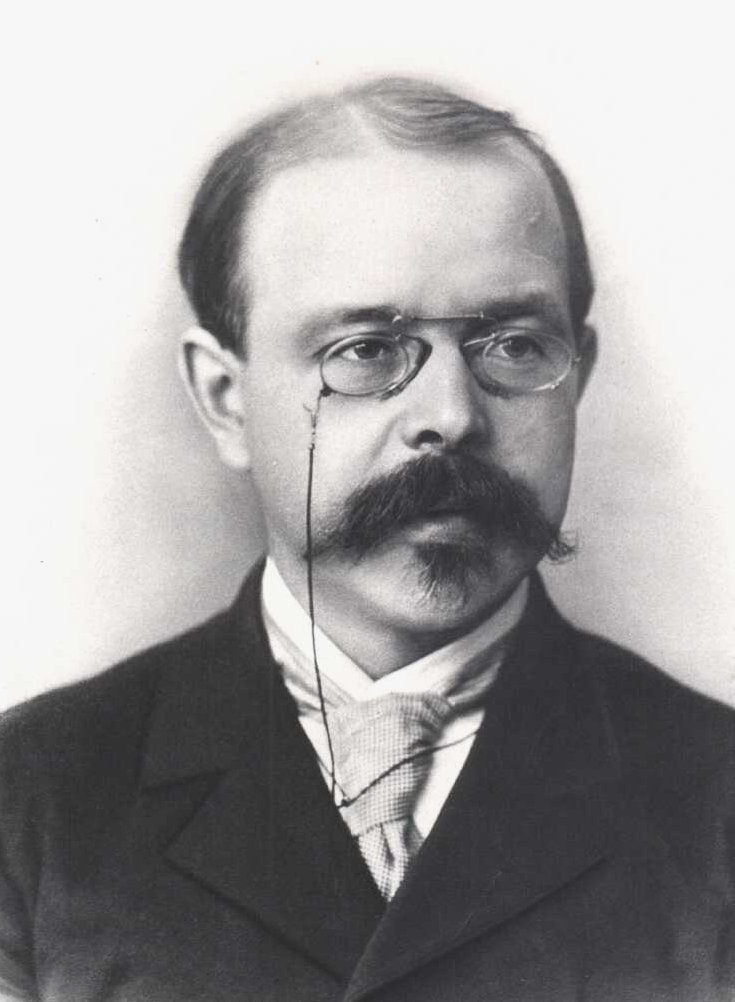
\includegraphics[width=\linewidth]{images/book2/nernst.jpg}
\end{minipage}\hfill
\begin{minipage}[t]{0.74\linewidth}\vspace{0pt}
वाल्टर नेर्न्स्ट (1864--1941), यहाँ पच्चीस वर्ष की आयु में, 1889 में। इस खंड का
समीकरण, जो किसी सेल की वोल्टता को उसके आयनों की सांद्रताओं से जोड़ता है,
उनके नाम पर है, और ऊष्मागतिकी का एक तीसरा सिद्धांत भी, जो द्वितीय वर्ष के
खंड में मिलता है। (छायाचित्र: स्मिथसोनियन
लाइब्रेरीज़, सार्वजनिक अधिकार-क्षेत्र, विकिमीडिया कॉमन्स।)
\end{minipage}
\end{history}

\section{अपचयोपचय अभिक्रियाओं का पूर्वानुमान}

\begin{method}[अपचयोपचय अभिक्रिया का पूर्वानुमान]\label{met:b1:nernst:predict-redox}
\begin{enumerate}
  \item युग्मों को \omterm{def:b1:nernst:electrode-potential}{मानक विभवों} के एक ऊर्ध्वाधर पैमाने पर रखिए,
        \omterm{def:b1:nernst:couple}{ऑक्सीकारक} बाईं ओर, \omterm{def:b1:nernst:couple}{अपचायक} दाईं ओर।
  \item उपस्थित सबसे प्रबल \omterm{def:b1:nernst:couple}{ऑक्सीकारक} (सबसे ऊँचा $E^\circ$) उपस्थित सबसे प्रबल
        \omterm{def:b1:nernst:couple}{अपचायक} (सबसे निम्न $E^\circ$) से अभिक्रिया करता है:
        \omterm{def:b1:nernst:couple}{ऑक्सीकारक} से नीचे \omterm{def:b1:nernst:couple}{अपचायक} तक, फिर ऊपर उत्पादों तक जाने वाला तीर
        यूनानी अक्षर गामा, $\gamma$, बनाता है।
  \item अभिक्रिया अनुकूल ($K > 1$) होती है जब \omterm{def:b1:nernst:couple}{ऑक्सीकारक} का युग्म
        \omterm{def:b1:nernst:couple}{अपचायक} के युग्म से ऊपर हो; व्यवहार में यह \omterm{def:b1:extent-q-and-k:quantitative}{मात्रात्मक} होती है जब
        एक विनिमित इलेक्ट्रॉन के लिए अंतर लगभग \qty{0.25}{V} से अधिक हो।
\end{enumerate}
\end{method}

\begin{omfigure}
\begin{tikzpicture}[font=\small, >={Stealth}, y=2.6cm]
  \draw[->, thick] (0,-1.0) -- (0,1.85) node[above] {$E^\circ$ (V)};
  \foreach \e/\o/\r in {-0.76/\ce{Zn^2+}/\ce{Zn}, 0/\ce{H+}/\ce{H2},
      0.34/\ce{Cu^2+}/\ce{Cu}, 0.77/\ce{Fe^3+}/\ce{Fe^2+},
      1.36/\ce{Cl2}/\ce{Cl-}, 1.51/\ce{MnO4-}/\ce{Mn^2+}} {
    \draw (-0.12,\e) -- (0.12,\e);
    \node[anchor=east] at (-0.25,\e) {\o};
    \node[anchor=west] at (0.25,\e) {\r};
    \node[anchor=west, black!55, font=\scriptsize] at (2.0,\e) {\e};
  }
  \node[omProp] at (-1.0,1.85) {ऑक्सीकारक};
  \node[omDef] at (1.1,1.85) {अपचायक};
  % the gamma: Cu2+ meets Zn below it on the other side
  \draw[omThm, very thick, ->, rounded corners=4pt] (-1.0,0.28) -- (-1.0,-0.42) -- (0.6,-0.70);
  \draw[omThm, thick, ->] (-0.5,0.40) to[bend left=40] (0.5,0.40);
  \draw[omThm, thick, ->] (0.5,-0.85) to[bend left=40] (-0.5,-0.85);
\end{tikzpicture}

{\small \omterm{def:b1:nernst:electrode-potential}{मानक विभवों} का एक पैमाना। गामा नियम: \omterm{def:b1:nernst:couple}{ऑक्सीकारक}
\ce{Cu^2+}, दूसरी ओर अपने नीचे स्थित \omterm{def:b1:nernst:couple}{अपचायक} \ce{Zn} से अभिक्रिया करता है
(मोटा तीर); \ce{Cu^2+}, \ce{Cu} में अपचित होता है (ऊपरी वक्र तीर) और
\ce{Zn}, \ce{Zn^2+} में ऑक्सीकृत (निचला वक्र तीर)। प्रतीप अभिक्रिया,
\ce{Cu} की \ce{Zn^2+} के साथ, अनुकूल नहीं है।}
\end{omfigure}

\begin{proposition}[मानक विभवों से साम्य स्थिरांक]\label{prop:b1:nernst:equilibrium-constant}
अभिक्रिया $\mathrm{Ox_1} + \mathrm{Red_2} \rightleftharpoons
\mathrm{Red_1} + \mathrm{Ox_2}$ के लिए, जो $n$ इलेक्ट्रॉनों का विनिमय करती है,
\[
  \log K = \frac{n\,(E^\circ_1 - E^\circ_2)}{0.059}\quad\text{\qty{25}{\celsius} पर} .
\]
\end{proposition}

\begin{proof}
साम्य पर दोनों युग्मों से बने सेल में कोई धारा नहीं बहती:
दोनों इलेक्ट्रोडों का विभव समान होता है, $E_1 = E_2$। हर एक का \omterm{thm:b1:nernst:nernst}{नेर्न्स्ट
समीकरण} समान $n$ के साथ लिखिए: $E^\circ_1 + \frac{0.059}{n}\log
\frac{a(\mathrm{Ox_1})}{a(\mathrm{Red_1})} = E^\circ_2 + \frac{0.059}{n}\log
\frac{a(\mathrm{Ox_2})}{a(\mathrm{Red_2})}$, इसलिए $\frac{n(E^\circ_1 -
E^\circ_2)}{0.059} = \log\frac{a(\mathrm{Red_1})a(\mathrm{Ox_2})}{a(\mathrm{Ox_1})
a(\mathrm{Red_2})} = \log K$, जहाँ \omterm{def:b1:extent-q-and-k:activity}{सक्रियताएँ} साम्य वाली हैं।
\end{proof}

डेनियल अभिक्रिया के लिए $\log K = 2(0.34 + 0.76)/0.059 = 37$: ज़िंक
कॉपर आयनों को पूर्णतः अपचित कर देता है। \ce{2Fe^3+ + 2I- <=> 2Fe^2+ + I2} के लिए
$\log K = 2(0.77 - 0.53)/0.059 = 8.1$। विधि की कसौटी इससे
निकलती है: $n = 1$ के साथ \qty{0.25}{V} का अंतर $K = 10^{4.2}$ देता है।

\begin{proposition}[विभवों का संयोजन]\label{prop:b1:nernst:combined-potentials}
यदि युग्म $\mathrm{A}/\mathrm{B}$ ($n_1$ इलेक्ट्रॉन) और
$\mathrm{B}/\mathrm{C}$ ($n_2$) मिलकर $\mathrm{A}/\mathrm{C}$
($n_3 = n_1 + n_2$) बनाते हैं, तो $n_3 E^\circ_3 = n_1 E^\circ_1 + n_2 E^\circ_2$।
विभव नहीं जुड़ते; इलेक्ट्रॉन-भारित विभव जुड़ते हैं।
\end{proposition}

\begin{proof}
A, B और C वाले विलयन में, जो एक इलेक्ट्रोड के साथ साम्य में हो,
तीनों युग्मों का विभव समान $E$ होता है। पहले के \omterm{thm:b1:nernst:nernst}{नेर्न्स्ट
समीकरण} को $n_1$ से और दूसरे के समीकरण को $n_2$ से गुणा करके जोड़िए:
B की \omterm{def:b1:extent-q-and-k:activity}{सक्रियता} कट जाती है और $(n_1 + n_2)E = n_1E^\circ_1 + n_2E^\circ_2 +
0.059\log\frac{a(\mathrm{A})}{a(\mathrm{C})}$, जो A/C के \omterm{thm:b1:nernst:nernst}{नेर्न्स्ट
समीकरण} का $n_3$ गुना है, कथित $E^\circ_3$ के साथ।
\end{proof}

कॉपर: $2E^\circ(\ce{Cu^2+}/\ce{Cu}) = 0.16 + 0.52 = 0.68$, इसलिए
$E^\circ(\ce{Cu^2+}/\ce{Cu}) = 0.34$~V, जैसा सारणी में है। चूँकि
$E^\circ(\ce{Cu+}/\ce{Cu}) > E^\circ(\ce{Cu^2+}/\ce{Cu+})$, कॉपर(I)
आयन स्वयं को ऑक्सीकृत और अपचित करता है, \ce{2Cu+ -> Cu^2+ + Cu}: वह
पानी में टिक नहीं पाता (\cref{ch:b1:e-ph-diagrams})।

\begin{proposition}[दूसरे प्रकार का इलेक्ट्रोड]\label{prop:b1:nernst:second-kind}
क्लोराइड विलयन में सिल्वर क्लोराइड से लेपित सिल्वर के तार का
विभव है
\[
  E = E^\circ(\ce{AgCl}/\ce{Ag}) - 0.059\log[\ce{Cl-}], \qquad
  E^\circ(\ce{AgCl}/\ce{Ag}) = E^\circ(\ce{Ag+}/\ce{Ag}) - 0.059\,\mathrm{p}K_s(\ce{AgCl}) .
\]
\end{proposition}

\begin{proof}
तार विलयन के \ce{Ag+} के साथ साम्य में है:
$E = E^\circ(\ce{Ag+}/\ce{Ag}) + 0.059\log[\ce{Ag+}]$, और सिल्वर क्लोराइड
$[\ce{Ag+}] = K_s/[\ce{Cl-}]$ तय करता है। प्रतिस्थापन से,
$E = E^\circ(\ce{Ag+}/\ce{Ag}) + 0.059\log K_s - 0.059\log[\ce{Cl-}]$।
\end{proof}

संख्यात्मक रूप से $0.80 - 0.059 \times 9.75 = 0.22$~V, सारणी का वह मान
जो गिब्ज़ ऊर्जाओं से स्वतंत्र रूप से प्राप्त हुआ था। ऐसा इलेक्ट्रोड
क्लोराइड मापता है, या, नियत क्लोराइड पर, संदर्भ का काम करता है।

\section{अभ्यास}

\begin{exercise}[$\star$]\label{exo:b1:nernst:1}
रेखांकित परमाणु की \omterm{def:b1:nernst:oxidation-number}{ऑक्सीकरण संख्या} बताइए: \ce{\underline{N}H3},
\ce{\underline{N}O3-}, \ce{\underline{S}O4^2-}, \ce{H2\underline{O}2},
\ce{\underline{Cr}2O7^2-}, \ce{\underline{Cl}O-}, \ce{\underline{Fe}3O4}
(औसत), \ce{\underline{C}H3OH}।
\end{exercise}

\begin{exercise}[$\star$]\label{exo:b1:nernst:2}
अम्ल में \ce{Cr2O7^2-}/\ce{Cr^3+},
\ce{H2O2}/\ce{H2O}, \ce{O2}/\ce{H2O2} और \ce{SO4^2-}/\ce{SO2} के \omterm{def:b1:nernst:couple}{अर्ध-समीकरण} संतुलित कीजिए।
\end{exercise}

\begin{exercise}[$\star$]\label{exo:b1:nernst:3}
\ce{Zn^2+}/\ce{Zn}, \ce{Cl2}/\ce{Cl-},
\ce{O2}/\ce{H2O} और \ce{Hg2Cl2}/\ce{Hg} का \omterm{thm:b1:nernst:nernst}{नेर्न्स्ट समीकरण} लिखिए। \qty{0.010}{mol/L}
ज़िंक सल्फ़ेट में ज़िंक की पट्टी का विभव परिकलित कीजिए।
\end{exercise}

\begin{exercise}[$\star$]\label{exo:b1:nernst:4}
एक डेनियल सेल में \qty{0.10}{mol/L} \ce{Zn^2+} और
\qty{0.010}{mol/L} \ce{Cu^2+} है। हर इलेक्ट्रोड का विभव, \omterm{def:b1:nernst:cell}{सेल
वोल्टता} परिकलित कीजिए, और बताइए कि कौन-सा इलेक्ट्रोड \omterm{def:b1:nernst:cell}{ऐनोड} है।
\end{exercise}

\begin{exercise}[$\star\star$]\label{exo:b1:nernst:5}
अम्ल में \ce{MnO4- + Fe^2+} को संतुलित कीजिए, उसका साम्य स्थिरांक परिकलित कीजिए और
बताइए कि क्या यह अनुमापन के काम आ सकती है।
\end{exercise}

\begin{exercise}[$\star\star$]\label{exo:b1:nernst:6}
इनमें से कौन-सी धातुएँ \qty{1}{mol/L} के ऐसे अम्ल में, जो स्वयं
\omterm{def:b1:nernst:couple}{ऑक्सीकारक} नहीं है (हाइड्रोक्लोरिक अम्ल), हाइड्रोजन देते हुए घुलती हैं: Mg, Zn, Fe, Ni,
Pb, Cu, Ag? अभिक्रियाएँ लिखिए और मैग्नीशियम तथा आयरन के लिए
$\log K$ परिकलित कीजिए।
\end{exercise}

\begin{exercise}[$\star\star$]\label{exo:b1:nernst:7}
आयोडीन अनुमापन \ce{I2 + 2S2O3^2- -> 2I- + S4O6^2-} का उपयोग करते हैं। सारणी से इसका
स्थिरांक परिकलित कीजिए। क्या यह \omterm{def:b1:extent-q-and-k:quantitative}{मात्रात्मक} है?
\end{exercise}

\begin{exercise}[$\star\star$]\label{exo:b1:nernst:8}
$E^\circ(\ce{Fe^2+}/\ce{Fe}) = -0.41$~V और $E^\circ(\ce{Fe^3+}/\ce{Fe^2+})
= 0.77$~V से $E^\circ(\ce{Fe^3+}/\ce{Fe})$ परिकलित कीजिए। दिखाइए कि आयरन(III) आयन
आयरन धातु से अभिक्रिया करते हैं, और स्थिरांक परिकलित कीजिए।
\end{exercise}

\begin{exercise}[$\star\star$]\label{exo:b1:nernst:9}
दिखाइए कि \qty{1}{bar}
ऑक्सीजन के अंतर्गत युग्म \ce{O2}/\ce{H2O} का विभव $1.23 - 0.059\,\mathrm{pH}$ है, और
\qty{1}{bar} हाइड्रोजन के अंतर्गत \ce{H+}/\ce{H2} का $-0.059\,\mathrm{pH}$। हाइड्रोजन--ऑक्सीजन
ईंधन सेल की वोल्टता क्या है? क्या यह pH पर निर्भर करती है?
\end{exercise}

\begin{exercise}[$\star\star\star$]\label{exo:b1:nernst:10}
कॉपर(I) आयन। सारणी की सहायता से दिखाइए कि \ce{Cu+} पानी में असमानुपातित
होता है, \ce{2Cu+ <=> Cu^2+ + Cu} का स्थिरांक परिकलित कीजिए, और \ce{Cu+} की
वह सांद्रता भी जो कॉपर धातु तथा \qty{0.10}{mol/L} \ce{Cu^2+} के साथ
साम्य में बचती है।
\end{exercise}

\begin{exercise}[$\star\star\star$]\label{exo:b1:nernst:11}
सेल \ce{Ag} $|$ \ce{Ag+} (\qty{1.0e-3}{mol/L}) $\|$ \ce{Ag+}
(\qty{0.10}{mol/L}) $|$ \ce{Ag} में दोनों ओर एक ही युग्म है।
इसकी वोल्टता परिकलित कीजिए, इसके ध्रुव पहचानिए और बताइए कि धारा देते समय
सांद्रताएँ कैसे बदलती हैं। यह कब रुकता है?
\end{exercise}

\begin{exercise}[$\star\star\star$]\label{exo:b1:nernst:12}
हाइड्रोजन परॉक्साइड। सारणी से
\ce{2H2O2 -> 2H2O + O2} का स्थिरांक परिकलित कीजिए और समझाइए कि हाइड्रोजन परॉक्साइड की बोतल
फिर भी महीनों तक स्थायी क्यों रहती है। सारणी का कौन-सा युग्म इसे
\omterm{def:b1:nernst:couple}{ऑक्सीकारक} बनाता है, कौन-सा \omterm{def:b1:nernst:couple}{अपचायक}?
\end{exercise}

\section{समस्या: क्लोराइड मापने वाला इलेक्ट्रोड}

\begin{problem}[{सप्ताहांत समस्या --- सिल्वर क्लोराइड युग्म की ऑक्सीकरण
संख्याएँ, हाइड्रोजन इलेक्ट्रोड के सापेक्ष एक सेल, पानी के एक नमूने के
क्लोराइड का मापन, और सिल्वर--सिल्वर क्लोराइड इलेक्ट्रोड का
मानक विभव}]
\label{pb:b1:nernst:1}
पानी की एक प्रयोगशाला सिल्वर क्लोराइड से लेपित सिल्वर के तार से क्लोराइड मापती है,
जिसे नमूने में डुबोकर एक \omterm{def:b1:nernst:reference-electrode}{संदर्भ इलेक्ट्रोड} से जोड़ा जाता है।
\qty{25}{\celsius} पर आँकड़े: $E^\circ(\ce{Ag+}/\ce{Ag}) = 0.80$~V,
$E^\circ(\ce{AgCl}/\ce{Ag}) = 0.22$~V, $E^\circ(\ce{Hg2Cl2}/\ce{Hg}) =
0.27$~V, $\mathrm{p}K_s(\ce{AgCl}) = 9.75$, $RT\ln 10/F = 0.059$~V,
$M(\ce{Cl}) = \qty{35.5}{g/mol}$।

\medskip
\noindent\textbf{भाग I --- युग्म।}
\begin{enumerate}
  \item Ag, \ce{Ag+} और \ce{AgCl} में सिल्वर की \omterm{def:b1:nernst:oxidation-number}{ऑक्सीकरण संख्या} बताइए,
        और \ce{AgCl} तथा \ce{Cl-} में क्लोरीन की।
  \item युग्म \ce{AgCl}/\ce{Ag} का \omterm{def:b1:nernst:couple}{अर्ध-समीकरण} लिखिए।
  \item इसका \omterm{thm:b1:nernst:nernst}{नेर्न्स्ट समीकरण} लिखिए।
  \item समझाइए कि विभव केवल क्लोराइड की
        सांद्रता पर क्यों निर्भर करता है।
  \item \qty{1.0}{mol/L}
        क्लोराइड में इलेक्ट्रोड का विभव क्या है?
  \item \qty{0.010}{mol/L} क्लोराइड में इसे परिकलित कीजिए।
\end{enumerate}

\medskip
\noindent\textbf{भाग II --- हाइड्रोजन इलेक्ट्रोड के सापेक्ष एक सेल।}
\begin{enumerate}[resume]
  \item \omterm{def:b1:nernst:electrode-potential}{मानक हाइड्रोजन इलेक्ट्रोड} और \qty{0.10}{mol/L} क्लोराइड में
        सिल्वर क्लोराइड इलेक्ट्रोड से बना सेल लिखिए।
  \item कौन-सा इलेक्ट्रोड धन ध्रुव है?
  \item \omterm{def:b1:nernst:cell}{सेल वोल्टता} परिकलित कीजिए।
  \item सेल के धारा देते समय चलने वाली अभिक्रिया लिखिए।
  \item इसका साम्य स्थिरांक परिकलित कीजिए।
  \item तार में इलेक्ट्रॉन किस दिशा में चलते हैं?
\end{enumerate}

\medskip
\noindent\textbf{भाग III --- क्लोराइड मापना।}
संदर्भ \qty{1.0}{mol/L} पोटैशियम क्लोराइड में एक कैलोमेल इलेक्ट्रोड
है।
\begin{enumerate}[resume]
  \item संदर्भ का विभव क्या है?
  \item \qty{1.0e-3}{mol/L} क्लोराइड वाले नमूने के लिए कौन-सा इलेक्ट्रोड
        धन ध्रुव है, और वोल्टता क्या है?
  \item वोल्टता $U$ (सिल्वर इलेक्ट्रोड घटा संदर्भ) को
        $[\ce{Cl-}]$ के फलन के रूप में व्यक्त कीजिए।
  \item एक नमूना $U = \qty{0.115}{V}$ देता है। उसकी क्लोराइड
        सांद्रता \unit{mol/L} और \unit{mg/L} में परिकलित कीजिए।
  \item $U$ पर \qty{1}{mV} की त्रुटि सांद्रता पर कितनी आपेक्षिक त्रुटि
        देती है?
  \item किस क्लोराइड सांद्रता से नीचे इलेक्ट्रोड \omterm{thm:b1:nernst:nernst}{नेर्न्स्ट समीकरण} का अनुसरण करना
        बंद कर देता है, क्योंकि उसका सिल्वर क्लोराइड घुलने लगता है?
\end{enumerate}

\medskip
\noindent\textbf{भाग IV --- 0.22 V कहाँ से आता है?}
\begin{enumerate}[resume]
  \item \ce{Ag+}/\ce{Ag} का \omterm{thm:b1:nernst:nernst}{नेर्न्स्ट समीकरण} लिखिए।
  \item ठोस सिल्वर क्लोराइड की उपस्थिति में $[\ce{Ag+}]$ को
        $[\ce{Cl-}]$ के फलन के रूप में व्यक्त कीजिए।
  \item सिल्वर के तार का विभव
        $[\ce{Cl-}]$ के फलन के रूप में निकालिए।
  \item इस व्यंजक में $E^\circ(\ce{AgCl}/\ce{Ag})$ पहचानिए।
  \item इसे $E^\circ(\ce{Ag+}/\ce{Ag})$ और $\mathrm{p}K_s$ से परिकलित कीजिए, और
        सारणी के मान से तुलना कीजिए।
  \item सिल्वर--सिल्वर क्लोराइड इलेक्ट्रोड का \omterm{def:b1:nernst:electrode-potential}{मानक विभव} दो दशमलव स्थानों तक
        बताइए।
\end{enumerate}
\end{problem}
